\documentclass[../../../analisi-dei-requisiti.tex]{subfiles}

\begin{document}


\begin{figure}[H]
  \centering
  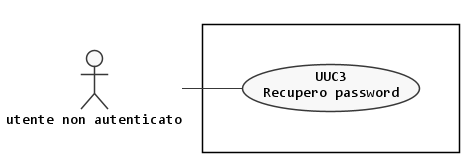
\includegraphics[width=100mm]{recupero-credenziali.png}
  \caption{UUC3: Recupero credenziali}%
  \label{fig:uuc3}
\end{figure}

\begin{description}
  \item[Caso d’uso:] UUC3;
  \item[Titolo:] Recupero credenziali;
  \item[Attori primari:] utente non autenticato;
  \item[Precondizione:] il sistema deve rendere disponibile la schermata di autenticazione;
  \item[Postcondizione:] l'utente si trova nella schermata di recupero credenziali;
  \item[Scenario principale:]
        \begin{enumerate}
          \item l’utente può selezionare la voce per il recupero credenziali che avviene tramite l'invio alla mail registrata di un link per reimpostare la sua password.
        \end{enumerate}
\end{description}

\subsubsection{UUC3.1: Recupero password}%
\label{subs:UUC3.1}

\begin{figure}[H]
  \centering
  \scalegraphics{recupero-password.png}
  \caption{UUC3.1: Recupero password}%
  \label{fig:uuc3_1}
\end{figure}

\begin{description}
  \item[Caso d’uso:] UUC3.1;
  \item[Titolo:] Recupero password;
  \item[Attori primari:] utente non autenticato;
  \item[Precondizione:] il sistema deve rendere disponibile la schermata di recupero credenziali;
  \item[Postcondizione:] l'utente ha recuperato le credenziali e può nuovamente autenticarsi;
  \item[Scenario principale:]
        \begin{enumerate}
          \item tramite questa procedura, l’utente ha la possibilità di reimpostare la password.
        \end{enumerate}
\end{description}

\subsubsection{UUC3.1.1: Inserimento email di registrazione}%
\label{subs:UUC3.1.1}
\begin{description}
  \item[Caso d’uso:] UUC3.1.1;
  \item[Titolo:] Inserimento email di registrazione;
  \item[Attori primari:] utente non autenticato;
  \item[Precondizione:] il sistema deve rendere disponibile la possibilità di inserire l'email di registrazione;
  \item[Postcondizione:] l'utente ha inserito correttamente la email di registrazione;
  \item[Scenario principale:]
        \begin{enumerate}
          \item l'utente si trova nella schermata per il recupero delle credenziali e inserisce l'email di registrazione.
        \end{enumerate}
  \item[Estensioni:]
        \begin{enumerate}
          \item se l'email inserita non è registrata nel database, allora verrà segnalato un errore~\ref{subs:UUC3.1.3}.
        \end{enumerate}
\end{description}

\subsubsection{UUC3.1.2: Reimpostazione password}%
\label{subs:UUC3.1.2}
\begin{description}
  \item[Caso d’uso:] UUC3.1.2;
  \item[Titolo:] Reimpostazione password;
  \item[Attori primari:] utente non autenticato;
  \item[Precondizione:] l'utente ha ricevuto il link presente nella email personale per reimpostare la password;
  \item[Postcondizione:] l'utente ha inserito correttamente la nuova password e ha recuperato le proprie credenziali;
  \item[Scenario principale:]
        \begin{enumerate}
          \item l'utente reimposta la password in una procedura che avviene in due passaggi:
                \begin{enumerate}
                  \item reset della vecchia password, non visibile all'utente;
                  \item inserimento della nuova password e la conferma della nuova password.
                \end{enumerate}
        \end{enumerate}
  \item[Estensioni:]
        \begin{enumerate}
          \item se la nuova password non rispetta determinati vincoli, verrà visualizzato un errore~\ref{subs:UUC3.1.3};
          \item se la nuova password e la sua conferma non coincidono tra loro, verrà visualizzato un errore~\ref{subs:UUC3.1.3}.
        \end{enumerate}
\end{description}

\subsubsection{UUC3.1.3: Informazioni recupero non valide}%
\label{subs:UUC3.1.3}

\begin{description}
  \item[Caso d’uso:] UUC3.1.3;
  \item[Titolo:] Informazioni recupero non valide;
  \item[Attori primari:] utente non autenticato;
  \item[Precondizione:] l'utente ha provocato un errore nella procedura di recupero credenziali;
  \item[Postcondizione:] l'applicazione mobile comunica all'utente l'errore;
  \item[Scenario principale:]
        \begin{enumerate}
          \item l'utente cerca di effettuare l'autenticazione con credenziali errate.
        \end{enumerate}
\end{description}

\end{document}
